\documentclass[a4paper, oneside, 12pt]{book}
\usepackage[italian]{babel}
\usepackage[T1]{fontenc}
\usepackage{hyperref}
\usepackage{graphicx}
\usepackage[dvipsnames]{xcolor}
\usepackage{geometry}
\usepackage{float}
\geometry{
a4paper,
margin=1in,
%total={6in,8in},
%left=20mm,
%top=0mm,
}

\begin{document}

\frontmatter

\title{Progetto ingegneria del software \\ "Lavoratori stagionali"}
\author{Enrico Bragastini \\ Davide Bianchini \\ Andrea Mafficini}
% \date{}
\maketitle

\tableofcontents

\chapter{Specifiche dei casi d'uso}

\section{Note generali}
% \subsection{Note generali} 
Si vuole progettare un sistema informatico di una agenzia che fornisce servizi di supporto alla ricerca
di lavoro stagionale. I lavoratori interessati possono iscriversi al servizio, rivolgendosi agli sportelli
dell’agenzia. Il sistema deve permettere la gestione delle anagrafiche e la ricerca di lavoratori
stagionali, nei settori dell’agricoltura e del turismo.
I responsabili del servizio, dipendenti dell’agenzia, inseriscono i dati dei lavoratori. Per ogni
lavoratore vengono memorizzati i dati anagrafici (nome, cognome, luogo e data di nascita,
nazionalità), indirizzo, recapito telefonico personale (se presente), email, le eventuali
specializzazioni/esperienze precedenti (bagnino, barman, istruttore di nuoto, viticultore,
floricultore), lingue parlate, il tipo di patente di guida e se automunito. Sono inoltre memorizzati i
periodi e le zone (comuni), per i quali il lavoratore è disponibile. Di ogni lavoratore si memorizzano
anche le informazioni di almeno una persona da avvisare in caso di urgenza: nome, cognome,
telefono, indirizzo email.
I dipendenti dell’agenzia devono autenticarsi per poter accedere al sistema e inserire i dati dei
lavoratori. Il sistema permette ai dipendenti dell’agenzia di aggiornare le anagrafiche con tutti i
lavori che i lavoratori stagionali hanno svolto negli ultimi 5 anni. Per ogni lavoro svolto vanno
registrati: periodo, nome dell’azienda, mansioni svolte, luogo di lavoro, retribuzione lorda
giornaliera. Per i dipendenti dell’agenzia si memorizzano i dati anagrafici, l’indirizzo email, il telefono
e le credenziali di accesso (login e password).
Una volta registrate le informazioni sui lavoratori, il personale dell’agenzia può effettuare ricerche
rispetto a possibili profili richiesti.
In particolare, il sistema deve permettere ai dipendenti di effettuare ricerche per lavoratore, per
lingue parlate, periodo di disponibilità, mansioni indicate, luogo di residenza, disponibilità di
auto/patente di guida. Il sistema deve permettere di effettuare ricerche complesse, attraverso la
specifica di differenti condizioni di ricerca (sia in AND che in OR).

\newpage
\section{Casi d'uso}
Per i dipendenti dell’agenzia vengono memorizzate delle informazioni tra le quali delle credenziali di accesso per accedere al sistema. Una volta fatto l’accesso il dipendente può inserire i dati dei lavoratori stagionali, modificarne le anagrafiche ed effettuare ricerche in base a dei profili (filtrare la ricerca). 

\begin{figure}[h!]
	\centering
	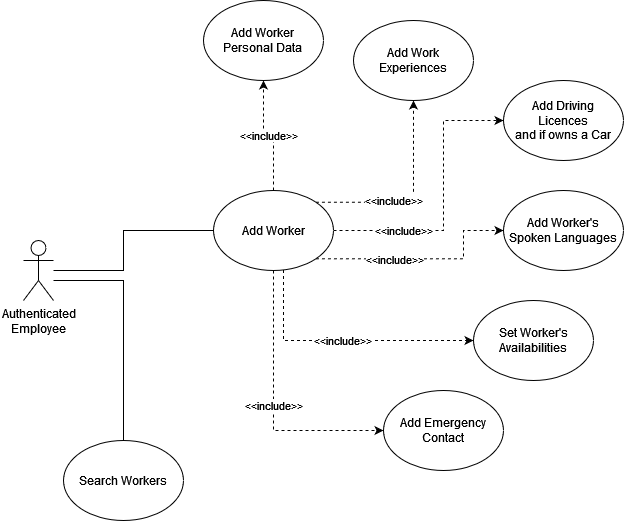
\includegraphics[width = 10 cm]{C:/Users/andre/Desktop/IngegneriaDelSoftwareProgetto/Documentazione/casiduso}
	% \caption{}
	\label{fig:casi d'uso}
\end{figure}

\subsection{Inserimento nuovo lavoratore}
I dipendenti dell’agenzia per poter effettuare l’inserimento e la gestione delle anagrafiche dei lavoratori è necessario che siano autenticati al sistema. \\

%\newgeometry{
%	a4paper,
	% total={170mm,257mm},
	% left=20mm,
	% top=10mm,
%}

\fbox{%
	\parbox{\textwidth}{%
		\textbf{Attori:} Dipendente dell’agenzia \\
		\textbf{Precondizioni:} Il dipendente deve essere autenticato. \\ 
		\textbf{Passi:}
		\begin{enumerate}
			\item Il dipendente accede al sistema
			\item Il dipendente è introdotto all’interfaccia di base
			\item Il dipendente compila il form con i dati anagrafici e il contatto di emergenza o modifica un form di un lavoratore esistente 
			\item Il dipendente inserisce il nuovo lavoratore o salva le modifiche del lavoratore modificato
		\end{enumerate}
		\textbf{Postcondizioni:}  Il lavoratore viene aggiunto dal database
	}%
}

\newpage
\subsection{Effettuare ricerche}
I dipendenti dell’agenzia per poter effettuare delle ricerche complesse è necessario che siano autenticati al sistema. \\
La ricerca può avvenire mediante una barra di testo tramite l’inserimento di nome e cognome.
\'E inoltre possibile filtrare ulteriormente i risultati in base a: lingue parlate, mansioni effettuate, periodo e comuni di disponibilità,
patenti di guida e disponibilità di auto propria. Tutti questi filtri possono inoltre essere applicati in modalità “AND” oppure “OR”. \\

\fbox{%
	\parbox{\textwidth}{%
		\textbf{Attori:} Dipendente dell’agenzia \\
		\textbf{Precondizioni:} Il dipendente deve essere autenticato. \\ 
		\textbf{Passi:}
		\begin{enumerate}
			\item Il dipendente accede al sistema
			\item Il dipendente è introdotto all’interfaccia di base
			\item Il dipendente visualizza la lista dei lavoratori
			\item Il dipendente filtra la lista dei lavoratori
		\end{enumerate}
	}%
}

\subsection{Cancellazione lavoratore}
I dipendenti dell’agenzia per poter cancellare un lavoratore è necessario che siano autenticati al sistema. \\
La cancellazione avviene tramite un pulsante dedicato per ogni lavoratore. \\

\fbox{%
	\parbox{\textwidth}{%
		\textbf{Attori:} Dipendente dell’agenzia \\
		\textbf{Precondizioni:} Il dipendente deve essere autenticato. \\ 
		\textbf{Passi:}
		\begin{enumerate}
			\item Il dipendente accede al sistema
			\item Il dipendente è introdotto all’interfaccia di base
			\item Il dipendente visualizza la lista dei lavoratori
			\item Il dipendente trova il lavoratore da eliminare
			\item Il dipendente elimina il lavoratore tramite apposito pulsante
		\end{enumerate}
		\textbf{Postcondizioni:}  Il lavoratore viene eliminato dal database
	}%
}

\newpage
\section{Diagrammi di attività}
\subsection{Autenticazione}
I dipendenti dell’agenzia per poter poter utilizzare il software è necessario che siano autenticati al sistema.

\begin{figure}[H]
	\centering
	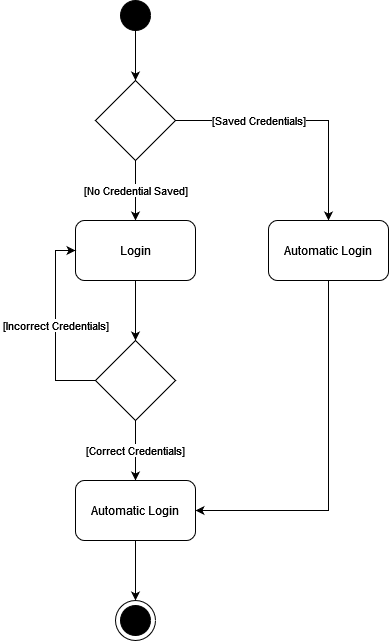
\includegraphics[width = 5 cm]{C:/Users/andre/Desktop/IngegneriaDelSoftwareProgetto/Documentazione/logincredenziali.png}
	% \caption{}
	\label{fig:login credenziali}
\end{figure}

\newpage
\subsection{Gestione delle anagrafiche}

\begin{figure}[H]
	\centering
	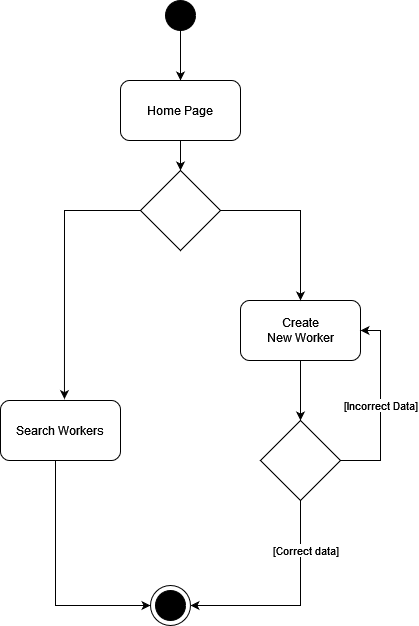
\includegraphics[width = 10 cm]{C:/Users/andre/Desktop/IngegneriaDelSoftwareProgetto/Documentazione/attivitadipendenti.png}
	% \caption{}
	\label{fig:attività dipendenti}
\end{figure}

Nota: i seguenti diagrammi catturano una singola attività di un utente rispetto al sistema. Non è stata rappresentata nel diagramma la possibilità di ripetere più volte la stessa operazione, in sequenza, senza chiudere il software. Questo per semplici ragioni di chiarezza e leggerezza; si considerano quindi le singole attività d’interazione

\end{document}

